\documentclass[letterpaper,11pt]{article}

\usepackage{float} % use with [H] to anchor figures
\usepackage[table,xcdraw]{xcolor}
\usepackage[open,openlevel=1]{bookmark}
\usepackage{amsmath}
\usepackage{graphicx}
\usepackage[ruled,vlined]{algorithm2e}
\usepackage{subcaption}
\setlength{\parindent}{0pt}
\hypersetup{pdfborder = {0 0 0}} % no colored links on table contents

\begin{document}




\title{Project 2: Backpropagation Neural Network\\
	\large MAT128B Winter 2020}
\author{Caitlin Brown}
\date{March 20, 2020}
\maketitle
\tableofcontents
\newpage

\section*{Introduction}

In this project, methods from numerical analysis, linear algebra and differential calculus come together to create an elementary backpropagation neural network. This particular network will learn to recognize handwritten digits. It will, so to speak, view an image, make some judgments, give a guess, evaluate its error, and adjust itself in such a way to improve its guess. Backpropagation then, in essence, refers to the gradient of how judgments (weights) are changed and the network 'learns'.


\section{MNIST Data Base}

The MNIST data base is a large collection of handwritten digits that take the form of highly standardized images. It is known for being particularly well-suited for neural networks and deep learning.\\

Below, code from the textbook "Numerical Methods" by Anne Greenbaum and Timothy P. Chartier is adapted to read in the data-frame and visualize a sample of digits from within it.\\

The format of the data-frame is 20 uint8 matrices. For digits 0 through 9, there are training and testing matrices, with the former containing many more rows. The rows of a matrix each represent data for one image. Therefore, we are provided with much more training data than testing data, in hopes that we will optimize our network. Each row is of length 784, containing integers that correspond to grayscale values. The code detailed below resizes a sample of such 1 by 784 vectors into 28 by 28 matrices. A grayscale colormap is then applied which generates 28 by 28 pixel images. 

\begin{figure}[]
	\centering
	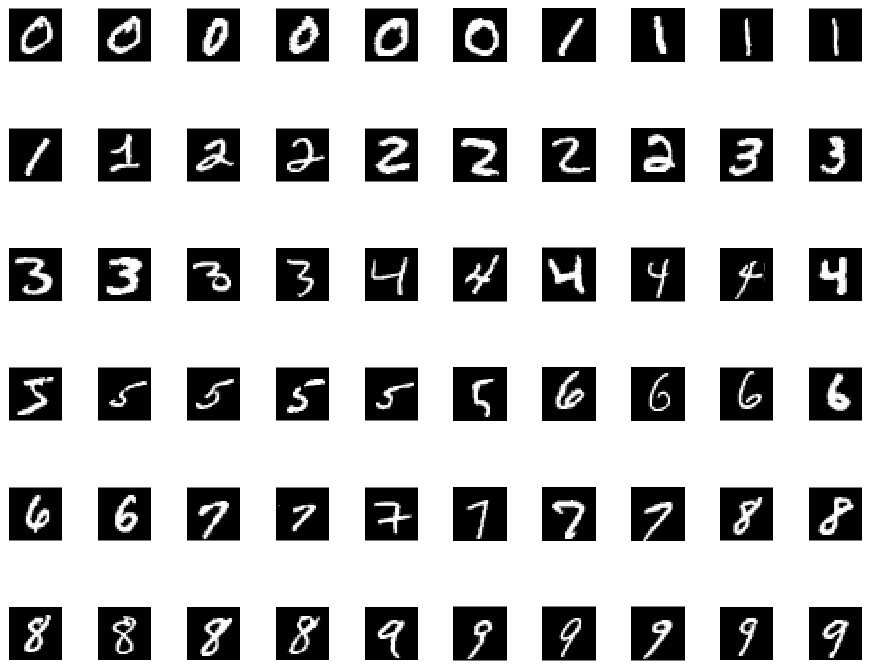
\includegraphics[width=4in]{fig3.png}
	\caption{Samples from MNIST data-frame}
	\label{fig:numbers}
\end{figure}

\vspace{5mm}
MATLAB Code:

\begin{verbatim}
load mnist_all.mat

zero = train0(1:6,:);
one = train1(1:6,:);
two = train2(1:6,:);
three = train3(1:6,:);
four = train4(1:6,:);
five = train5(1:6,:);
six = train6(1:6,:);
seven = train7(1:6,:);
eight = train8(1:6,:);
nine = train9(1:6,:);
numbers = [zero; one; two; three;...
    four; five; six; seven; eight; nine];

for i=1:length(numbers)
    subplot(6,10,i)
    pics = reshape(numbers(i,:),28,28);
    image(rot90(flipud(pics),-1)),
    colormap(gray(256)), axis square tight off;
end
\end{verbatim}



\section{Plot Digits}



Averages from the training data-frame are visualized. I created a matrix with 10 rows, one for each digit 0 through 9, and assigned each row with a calculation of the mean for a digit dataset. I then applied the same grayscale color-mapping as above and used the subplot function in MATLAB to visualize the results in a 2 by 5 format.

\begin{figure}[]
	\centering
	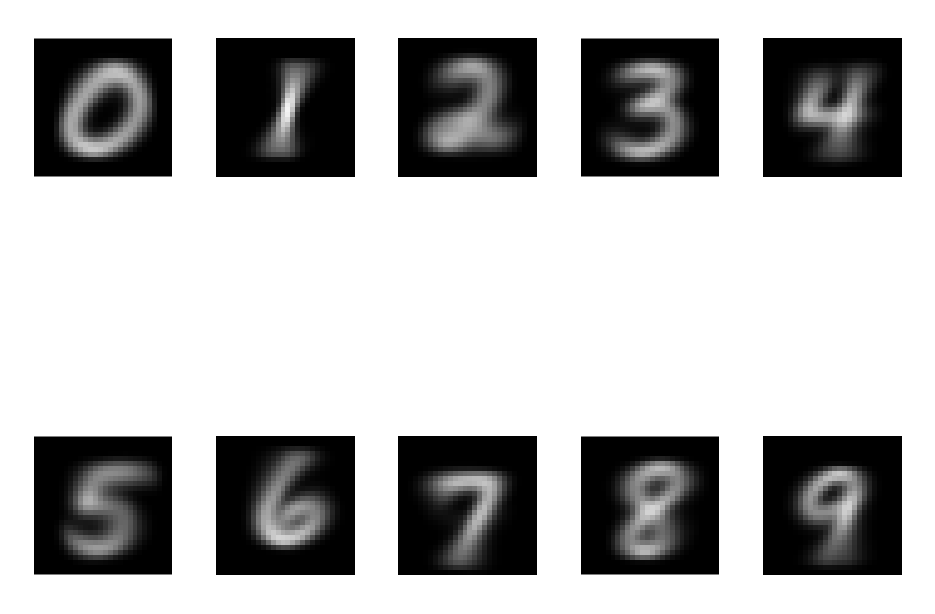
\includegraphics[width=2.5in]{fig2.png}
	\caption{Visualization of digit averages}
	\label{fig:averages}
\end{figure}

\vspace{5mm}
MATLAB Code:

\begin{verbatim}
T = zeros(10,784); % preallocate memory

T(1,:) = mean(train0);
T(2,:) = mean(train1);
T(3,:) = mean(train2);
T(4,:) = mean(train3);
T(5,:) = mean(train4);
T(6,:) = mean(train5);
T(7,:) = mean(train6);
T(8,:) = mean(train7);
T(9,:) = mean(train8);
T(10,:) = mean(train9);

for i = 1:10
    subplot(2,5,i)
    avgPic = T(i,:);
    avgPicImage = reshape(avgPic,28,28);
    image(rot90(flipud(avgPicImage),-1)),
    colormap(gray(256)), axis square tight off;
end
\end{verbatim}



\section{A Neuron}



To prepare for the upcoming task of implementing a full neural network, I laid the groundwork for a single "neuron". As stated in the project description, each neuron consists of two steps: a set of weighted connections, and an internal activation function. For the first step, local function \emph{computeNET} is defined to sum up the products of inputs and weights. For the second step, in this case, we are using the sigmoid function: \[f(x)=\frac{1}{1 + e^{-x}}\]
Named so because of its "S" shape between two horizontal asymptotes, 0 and 1. This is why we choose this function: it's output will always be in that interval, therefore it will scale our weighted sum into a more useful proportion. In the code below, some simple test data are included as comments.\\

\vspace{5mm}
MATLAB Code:

\begin{verbatim}
% inputs=[1 2]; inputWeights=[3 4];      % test data
% NET=computeNET(inputs,inputWeights);
% OUT=f(NET)

function NET = computeNET(inputs, inputWeights)
NET = sum(inputs.*inputWeights)
end

function OUT = f(NET)
OUT = 1/(1 + exp(-NET)) % sigmoid activation function
end
\end{verbatim}


\subsection{Verify Derivative of Sigmoid Function}

I used MATLAB to calculate this derivative as follows:\\

\begin{verbatim}
syms x
f = 1/(1 + exp(-x));
diff(f)

% ans =
%
% exp(-x)/(exp(-x) + 1)^2
\end{verbatim}

Now,


\[\frac{d}{dx} \frac{1}{1 + e^{-x}} = \frac{e^{-x}}{{(1 + e^{-x})}^2} = \frac{1}{1 + e^{-x}} - \frac{1}{{(1 + e^{-x})}^2} = \frac{1}{1 + e^{-x}}\left(1 - \frac{1}{1 + e^{-x}}\right)\]\

$= f(1-f)$

\vspace{5mm}
...which will be a convenient result later.



\section{Multilayer Network}

My MATLAB custom function \emph{multiLayerNetwork} makes use of the node created in the previous section and expands on it greatly. Here and in the next section, where I initialize weights, I lay down all the infrastructure needed for the network to make a forward pass.\\

The function takes as inputs: training data, weights and the user's chosen number of hidden layers. Its outputs: a cell containing the outputs of each hidden layer (to be used later in backpropagation), and of course the network's guess at what the digit is. The latter is actually the end layer in the aforementioned cell array. The network's guess is in the format of a 10 by 1 array, each element a value between [0,1] representing a percentage of confidence that the input digit is the one corresponding to that index in the array. For example, if the network were 100 percent certain that the digit was a zero and not any other number, then the returned array would have a 1 in the first index (because MATLAB begins indexing at 1) and 0's in the other nine indices.\\

Note in the code below, local functions (neuron functions from (3)) are modified to accommodate and produce harmonious matrices. Please note as well that variable \emph{weights} is to be explicitly defined in the next section.

\vspace{5mm}
MATLAB Code:

\begin{verbatim}

function [x, output] = multiLayerNetwork(input, weights, nHidLayers)
x = cell(1,nHidLayers+2);
x(1) = {input};

    for i=1:(nHidLayers+1)
    x(i+1) = {computeNET(x{i}, weights{i})};
    x(i+1) = {f(x{i+1})};
    end
    
output = x{end};
end

% Local fxns:
function NET = computeNET(inputs, inputWeights)
NET = inputWeights*inputs;
end

function OUT = f(NET)
OUT = 1./(1 + exp(-NET));
end

\end{verbatim}



\section{Initializing the Network}

In preparation for the first forward pass of the network, all the weights must be initialized to random small values. These values must be both positive and negative, per the project instructions. To accomplish this, I wrote another custom function in MATLAB called \emph{initialize}. Each node must have a weight, so naturally this function receives as inputs: number of hidden layers \emph{nHidLayers} and number of nodes \emph{nNeurons}, both up to the discretion of the user. What is generated is a cell array, each layer a matrix of weights corresponding to a hidden layer, which will be multiplied against the incoming data for that respective layer.\\

Iterative matrix multiplication of this magnitude, as any student of linear algebra would imagine, is a delicate process. All dimensions and inside/outside products must be calibrated just so. This function will generate weight matrices of dimension (outgoing data height x incoming data height) in preparation for right multiplication with incoming data (always a column vector). The initial vector of incoming data must be 784 entries long, and the last vector of outgoing data must be 10 entries long--it is the network's guess at the digit, as discussed earlier. All weight matrices corresponding to hidden layers are square with length \emph{nNeurons}.\\


\vspace{5mm}
MATLAB Code:

\begin{verbatim}
function weights = initialize(nHidLayers, nNeurons)

weights = cell(1, nHidLayers + 1);
weights(1) = {rand(nNeurons,784)-0.5};
weights(2:(end-1)) = {rand(nNeurons,nNeurons)-0.5};
weights(end) = {rand(10,nNeurons)-0.5};

end
\end{verbatim}



\section{Training the Network}

Now that all the pieces have been built, the stage is nearly set to train the network. Some adjustments need to be added to the script:\\

\emph{i.} Reformat the input. The network has access to a huge library of training samples. I leave it up to the user to declare how many samples from each digit data-base they would like to run--knowing of course that the network will execute a total of that number multiplied by 10 iterations. Using this assigned number \emph{samples}, the script generates a 1 by 10 cell array \emph{inputCell} with each layer a matrix containing a randomly selected arrangement of the detailed number of digit samples. From here, a for-loop is used to feed all the digit "images" into the algorithm, one at a time. Digit data comes in as a row from a uint8 matrix, and so needs to be converted to a 784 by 1 column array of type: double-precision floating-point number.\\

\emph{ii.} Assign the targets. Because the network will have 10 different targets over the course of its training, I defined a 10 by 10 identity matrix called \emph{targetMatrix} from which one column will be considered at a time and referred to as \emph{target}. Next, name and assign variable \emph{err} to be the difference (not absolute value) between the target and the network's guess.\\

\emph{iii.} Impose a training rate coefficient $\eta \in$ [0.01, 0.1] (aptly named \emph{eta} in code below). Choosing a smaller value for $\eta$ here slows down the algorithm's learning rate and increases the chances it will zero in on the optimal weight configuration. Choosing a value that is too high risks overshooting the minimum value of the error function (i.e. network won't "learn").\\

The algorithm is now ready for a forward pass. Once an output is given, the weights need to be adjusted. That is, the network needs to be backpropagated.\\

The first step toward achieving this is to take the result of the error function and use it to generate an array $\delta$ (named \emph{deltaOut} below). Referencing the derivative calculated in (3.1), $\delta$ will be equal to \emph{err} multiplied by the derivative of the sigmoid function for every element of the output array. This method of using the partial derivative of the activation function to minimize the error is known as stochastic gradient descent. These values are then further multiplied by the output of the connected node in the previous hidden layer, as well as $\eta$. This array, finally, is added to the weights generating the output layer, changing them.\\

The process for calculating $\delta$ for the hidden layers is slightly different. In essence, the $\delta$ from the layer previously propagated is utilized. This is why the method is referred to as "backpropagation"--all weight layers must be addressed in reverse order back to the beginning, at which time the network is primed for another forward pass, and hopefully more learning.

\vspace{5mm}
MATLAB Code:

\begin{verbatim}

load mnist_all.mat

samples = 1500;
selectSamples = randi(5400,samples,1);
inputCell = {...
    double(train0(selectSamples,:))',...
    double(train1(selectSamples,:))',...
    double(train2(selectSamples,:))',...
    double(train3(selectSamples,:))',...
    double(train4(selectSamples,:))',...
    double(train5(selectSamples,:))',...
    double(train6(selectSamples,:))',...
    double(train7(selectSamples,:))',...
    double(train8(selectSamples,:))',...
    double(train9(selectSamples,:))',...
    };

targetMatrix = eye(10);
guess = zeros(10);
nHidLayers = 5; 
nNeurons = 50;
weights = initialize(nHidLayers, nNeurons);
eta = 0.01;

for k=1:10
    inputMatrix = inputCell{k}; % select matrix
    target = targetMatrix(:,k);

    for j=1:samples
        input = inputMatrix(:,j); % cycle thru cols
    
        [x,output] = multiLayerNetwork(input, weights, nHidLayers);
        err = target - output;
        deltaOut = zeros(size(output)); % preallocate

        for i=1:length(output) % d/dx sigmoid * error
            deltaOut(i) = f(output(i)).*(1-f(output(i))).*(err(i));
        end

        delta = cell(size(weights));
        delta(end) = {deltaOut};

        for i = length(weights):-1:2
   
            delta{i-1} = zeros(size(x{i-1})); % preallocate
            delta{i-1} = sum(weights{i}'*delta{i})*...
                (f(x{i-1}).*(1-f(x{i-1})));

            weights{i} = weights{i} + eta*delta{i}*x{i}';
        end    
    end
    
    guess(:,k) = output;
end

disp('~Results~')
for l=1:10
    disp('Target:');disp(l-1)
    disp('Network''s guess:');disp(guess(:,l))
end

% local fxns
function OUT = f(NET)
OUT = 1./(1 + exp(-NET));
end

\end{verbatim}

\section{Dependence on Parameters}

It took numerous iterations (pun intended) of code writing to get a network architecture that could oblige a variable number of nodes and hidden layers. It meant starting from a bare-bones framework and gradually increasing the complexity.\\

...However, it was worth it because now, in this final stage, I can manipulate these parameters to optimize the network's outputs and enjoy the fruits of my labor.\\

Doing just that, I have observed a remarkable accuracy from the parameters in the code of the previous section. That is:\\

1500 samples of each digit 0-9\\
5 hidden layers\\
50 nodes\\
$\eta$ = 0.01\\

The guess for each digit obtained from these parameters is organized in the table below:



\begin{table}[H]
\centering
\begin{tabular}{l|lllll}
Digit  & 0                             & 1                             & 2                             & 3                             & 4                             \\ \hline
Output & {\color[HTML]{3531FF} 0.9931} & 0.0056                        & 0.0027                        & 0.0018                        & 0.0014                        \\
       & 0.0059                        & {\color[HTML]{3531FF} 0.993}  & 0.0056                        & 0.0027                        & 0.0018                        \\
       & 0.0052                        & 0.0026                        & {\color[HTML]{3531FF} 0.9929} & 0.0056                        & 0.0027                        \\
       & 0.0055                        & 0.0027                        & 0.0018                        & {\color[HTML]{3531FF} 0.9929} & 0.0056                        \\
       & 0.0058                        & 0.0028                        & 0.0018                        & 0.0014                        & {\color[HTML]{3531FF} 0.9929} \\
       & 0.0058                        & 0.0028                        & 0.0018                        & 0.0014                        & 0.0011                        \\
       & 0.0055                        & 0.0027                        & 0.0018                        & 0.0013                        & 0.0011                        \\
       & 0.0061                        & 0.0028                        & 0.0019                        & 0.0014                        & 0.0011                        \\
       & 0.0036                        & 0.0022                        & 0.0015                        & 0.0012                        & 0.001                         \\
       & 0.006                         & 0.0028                        & 0.0019                        & 0.0014                        & 0.0011                        \\
       &                               &                               &                               &                               &                               \\
Digit  & 5                             & 6                             & 7                             & 8                             & 9                             \\ \hline
Output & 0.0011                        & 0.0009                        & 0.0008                        & 0.0007                        & 0.0006                        \\
       & 0.0014                        & 0.0011                        & 0.0009                        & 0.0008                        & 0.0007                        \\
       & 0.0018                        & 0.0014                        & 0.0011                        & 0.0009                        & 0.0008                        \\
       & 0.0027                        & 0.0018                        & 0.0014                        & 0.0011                        & 0.0009                        \\
       & 0.0056                        & 0.0027                        & 0.0018                        & 0.0014                        & 0.0011                        \\
       & {\color[HTML]{3531FF} 0.9929} & 0.0056                        & 0.0027                        & 0.0018                        & 0.0014                        \\
       & 0.0009                        & {\color[HTML]{3531FF} 0.9929} & 0.0056                        & 0.0027                        & 0.0018                        \\
       & 0.0009                        & 0.0008                        & {\color[HTML]{3531FF} 0.9929} & 0.0056                        & 0.0027                        \\
       & 0.0008                        & 0.0007                        & 0.0006                        & {\color[HTML]{3531FF} 0.9929} & 0.0056                        \\
       & 0.0009                        & 0.0008                        & 0.0007                        & 0.0006                        & {\color[HTML]{3531FF} 0.9929}
\end{tabular}
\end{table}

That was for training data. Now, using testing data and these parameters:\\

890 samples of each digit 0-9\\
5 hidden layers\\
50 nodes\\
$\eta$ = 0.01\\

The following data are returned:\\

\begin{table}[H]
\centering
\begin{tabular}{l|lllll}
Digit  & 0                             & 1                             & 2                             & 3                             & 4                             \\ \hline
Output & {\color[HTML]{3531FF} 0.9888} & 0.0086                        & 0.0042                        & 0.0027                        & 0.002                         \\
       & 0.0054                        & {\color[HTML]{3531FF} 0.9892} & 0.0086                        & 0.0042                        & 0.0027                        \\
       & 0.0082                        & 0.0041                        & {\color[HTML]{3531FF} 0.9892} & 0.0086                        & 0.0042                        \\
       & 0.0018                        & 0.0015                        & 0.0013                        & {\color[HTML]{3531FF} 0.9891} & 0.0086                        \\
       & 0.0078                        & 0.004                         & 0.0026                        & 0.002                         & {\color[HTML]{3531FF} 0.9891} \\
       & 0.0084                        & 0.0041                        & 0.0027                        & 0.002                         & 0.0016                        \\
       & 0.0092                        & 0.0043                        & 0.0028                        & 0.0021                        & 0.0016                        \\
       & 0.0081                        & 0.004                         & 0.0027                        & 0.002                         & 0.0016                        \\
       & 0.0085                        & 0.0041                        & 0.0027                        & 0.002                         & 0.0016                        \\
       & 0.0081                        & 0.004                         & 0.0027                        & 0.002                         & 0.0016                        \\
       &                               &                               &                               &                               &                               \\
Digit  & 5                             & 6                             & 7                             & 8                             & 9                             \\ \hline
Output & 0.0016                        & 0.0014                        & 0.0012                        & 0.001                         & 0.0009                        \\
       & 0.002                         & 0.0016                        & 0.0014                        & 0.0012                        & 0.001                         \\
       & 0.0027                        & 0.002                         & 0.0016                        & 0.0014                        & 0.0012                        \\
       & 0.0042                        & 0.0027                        & 0.002                         & 0.0016                        & 0.0014                        \\
       & 0.0086                        & 0.0042                        & 0.0027                        & 0.002                         & 0.0016                        \\
       & {\color[HTML]{3531FF} 0.9891} & 0.0086                        & 0.0042                        & 0.0027                        & 0.002                         \\
       & 0.0014                        & {\color[HTML]{3531FF} 0.9891} & 0.0086                        & 0.0042                        & 0.0027                        \\
       & 0.0013                        & 0.0011                        & {\color[HTML]{3531FF} 0.9891} & 0.0086                        & 0.0042                        \\
       & 0.0013                        & 0.0012                        & 0.001                         & {\color[HTML]{3531FF} 0.9891} & 0.0086                        \\
       & 0.0013                        & 0.0011                        & 0.001                         & 0.0009                        & {\color[HTML]{3531FF} 0.9891}
\end{tabular}
\end{table}


\section{Conclusion}

My final data are pretty exciting, I think. My network is telling me that it judges my inputs correctly 98 or 99 percent of the time. Looking back at Figure 1, the variety of handwriting styles only serves to make this more impressive. I remember back when I was writing my script to initialize the weights--I would run it to check if it was working and a totally random output guess would be generated with positive and negative rational numbers between [-1,1]. To go from that to one of the output arrays detailed above is a massive achievement.\\

Artificial neural networks like this one are clearly inspired by the organic neural networks that are our brains. This particular example is known as a feedforward network, which is generally considered to be the simplest prototype. Convolutional neural networks, like the famous AlphaGo of 2015 are another flavor of this type of network. There are also other more complicated prototypes, such as ones that have a "memory" to learn differently, ones that impose statistical randomness upon themselves, and even modular ones that are more closely modeled after the architecture of the human brain (specialized areas for vision, touch, abstract thinking, etc.)\\

As we learn more about ourselves and our technology this is an exciting area of research.

\section{Appendix}
\subsection{Group Work}

I (Caitlin) did this whole project by myself! It was an epic amount of work and I'm proud of myself, particularly considering I hadn't used MATLAB or even written code at all before this quarter--I've learned a lot in this class.\\

After the first project on fractal geometry, one team member decided to migrate to another group. The other and I agreed to stay together for project two, and seek out a new third member. We were clearly unsuccessful in that endeavor. I have a GitHub repository for this project which I have been regularly updating over the course of the last few weeks. I invited my teammate as a contributor and kindly asked them to inform me of any difficulty they had in cloning, committing, etc. We had email correspondence for a while where I would summarize my progress to them, and they would say they were planning on working on it, or going to office hours. I would follow up to find they hadn't.\\

I felt bad to leave their name off the final draft, as we'd agreed to be a team. However, it also felt wrong to include their name on a project that I labored on for weeks and that they contributed literally 0 percent to. I'm not upset: I had fun getting this to work and I'm grateful that I was able to learn so much about neural nets in an undergrad class. I expect it to be a useful base to build upon in the future.

\subsection{GitHub}

Here is the URL for my GitHub repository:\\

https://github.com/caibrown/MAT128B-Project2

\end{document}
